\documentclass[tikz, border=4pt]{standalone}

% --- packages (mirror these in kcl-node.meta.json "requires") ---
\usepackage{tikz}
\usetikzlibrary{positioning}

% --- palette (canonical source: reference/color-palettes/color-palettes.md; light variant) ---
\definecolor{otgray}{HTML}{5A5A5A}
% --- ESL domain-semantic tokens (contract §2, ADR-0005 D7) ---
\colorlet{analogdomain}{orange}

\begin{document}
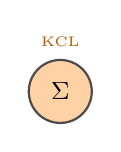
\begin{tikzpicture}
  % contract §1a `kcl-node`: "summation node collecting column current;
  % ALWAYS tagged 'KCL'" -- the small caption above the node is not
  % decoration, it is the component's contract-mandated tag.
  \node[circle, draw=otgray!85!black, thick, fill=analogdomain!35,
        minimum size=8mm, inner sep=0pt, font=\small] (kcl) {$\Sigma$};
  \node[font=\tiny, text=analogdomain!70!black, above=1pt of kcl] {KCL};
\end{tikzpicture}
\end{document}
